\documentclass[specification,annotation,times]{itmo-student-thesis}

%% Опции пакета:
%% - specification - если есть, генерируется задание, иначе не генерируется
%% - annotation - если есть, генерируется аннотация, иначе не генерируется
%% - times - делает все шрифтом Times New Roman, требует пакета pscyr.

%% Делает запятую в формулах более интеллектуальной, например:
%% $1,5x$ будет читаться как полтора икса, а не один запятая пять иксов.
%% Однако если написать $1, 5x$, то все будет как прежде.
\usepackage{icomma}

%% Данные пакеты необязательны к использованию в бакалаврских/магистерских
%% Они нужны для иллюстративных целей
%% Начало
\usepackage{tikz}
\usetikzlibrary{arrows}
\usepackage{filecontents}
\usepackage{wrapfig}

%% Указываем файл с библиографией.
\addbibresource{master-thesis.bib}

\begin{document}

\studygroup{M4239}
\title{Анализ и разработка алгоритмов сжатия коротких текстов}
\author{Минаев Борис Юрьевич}{Минаев Б.Ю.}
\supervisor{Буздалов Максим Викторович}{Буздалов М.В.}{канд. техн. наук}{доцент кафедры компьютерных технологий Университета ИТМО}
\publishyear{2017}
%% Дата выдачи задания. Можно не указывать, тогда надо будет заполнить от руки.
\startdate{01}{сентября}{2015}
%% Срок сдачи студентом работы. Можно не указывать, тогда надо будет заполнить от руки.
%\finishdate{31}{мая}{2015}
%% Дата защиты. Можно не указывать, тогда надо будет заполнить от руки.
%\defencedate{15}{июня}{2015}

%\addconsultant{Белашенков Н.Р.}{канд. физ.-мат. наук, без звания}
%\addconsultant{Беззубик В.В.}{без степени, без звания}

\secretary{Павлова О.Н.}

%% Задание
%%% Техническое задание и исходные данные к работе
\technicalspec{Требуется проанализировать существующие алгоритмы сжатия текстовых данных. Оценить их применимость к сжатию коротких текстовых сообщений, посылаемых в социальных сетях. 
Реализовать собственный алгоритм сжатия текстовых сообщений, который можно было бы применить для уменьшения объемов используемой памяти на серверах, которые хранят текстовые сообщения. }

%%% Содержание выпускной квалификационной работы (перечень подлежащих разработке вопросов)
\plannedcontents{
    \begin{enumerate}
        \item изучение существующих алгоритмов сжатия текстовых данных;
        \item изучение особенностей посылаемых в социальных сетях текстовых сообщений с точки зрения их сжатия;
        \item разработка нового алгоритма сжатия;
        \item сравнение полученного алгоритма и существующих решений;
        \item выводы
    \end{enumerate}

}

%%% Исходные материалы и пособия 
\plannedsources{\begin{enumerate}
    \item Б.Д.Кудряшов. Основы теории кодирования
    \item Salomon D., Motta G. Handbook of Data Compression
\end{enumerate}}

%%% Календарный план
\addstage{Изучение существующих алгоритмов сжатия}{12.2015}
\addstage{Изучение особенностей данных}{03.2016}
\addstage{Применение существующих алгоритмов, выяснение их достоинств и недостатков}{06.2016}
\addstage{Разработка собственного алгоритма, сравнение с аналогами}{03.2017}
\addstage{Написание пояснительной записки}{05.2017}

%%% Цель исследования
\researchaim{Разработка алгоритма сжатия коротких текстовых сообщений}

%%% Задачи, решаемые в ВКР
\researchtargets{\begin{enumerate}
    \item уменьшение количества памяти, необходимое для хранение текстовых сообщений
    \item увеличиние скорости считывания сообщений с диска
\end{enumerate}}

%%% Использование современных пакетов компьютерных программ и технологий
\advancedtechnologyusage{
Для сравнения алгоритмов сжатия, они были реализованы на языке программирования Java. 
Разработанный алгоритм был переписан на язык C для увеличения скорости его работы.
Для написания автоматических тестов был использован язык PHP. Для визуализации данных 
был использован Python и matplotlib.
}

%%% Краткая характеристика полученных результатов 
\researchsummary{
Был разработан алгоритм сжатия коротких текстовых сообщений, который был применен в ООО <<В Контакте>>. 
По сравнению с предыдущим используемым алгоритмом размер сжатых сообщений уменьшился на 5-7\%. 
Такое улучшение соответствует экономии нескольких терабайт оперативной памяти на масштабах ООО <<В Контакте>>
}

%%% Гранты, полученные при выполнении работы 
\researchfunding{Грантов получено не было.}

%%% Наличие публикаций и выступлений на конференциях по теме выпускной работы
\researchpublications{
Публикаций подготовлено не было.
}	

%% Эта команда генерирует титульный лист и аннотацию.
\maketitle{Магистр}

%% Оглавление
\tableofcontents


%% Макрос для введения. Совместим со старым стилевиком.
\startprefacepage

В последнее время количество информации во всем мире стремительно увеличивается. 
Согласно \cite{two-times} за каждые два года суммарное количество данных в интернете увеличивается в два раза. 
Аналогичные результаты подтверждаются исследованиями, которые были проведены автором во время работы в компании ВКонтакте. 
Эта компания владеет одноименным сайтом, на котором пользователи могут обмениваться сообщениями. 
На рис.~\ref{fig1} показано количество сообщений, отправленных пользователями в течении разных месяцев. 
Эти данные заставили задуматься о пересмотре архитектуры хранения сообщений, а также улучшении эффективности их обработки.

\begin{figure}[h!]
  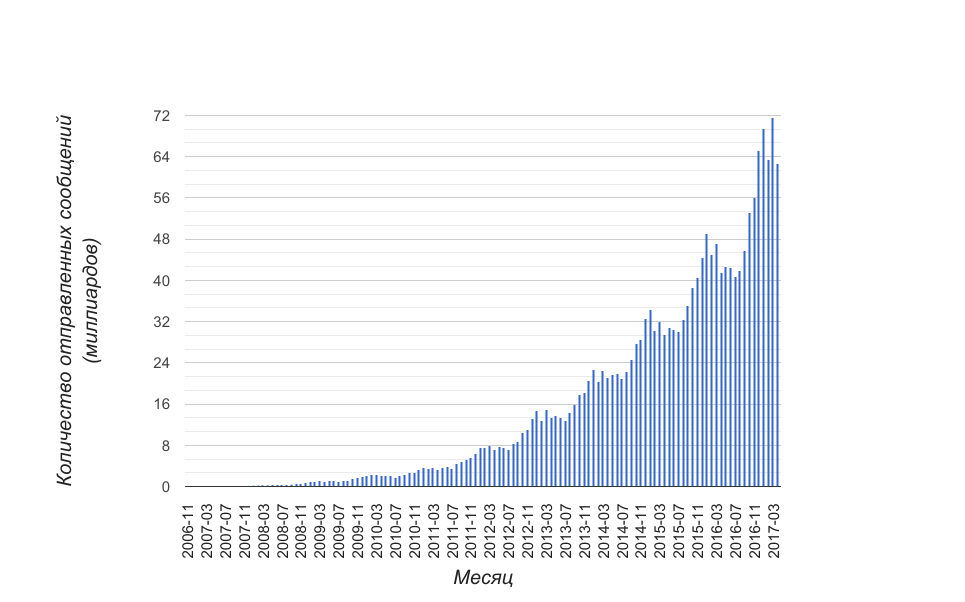
\includegraphics[width=\linewidth]{pics/msgs-num.png}
  \caption{Количество отправляемых сообщений}
  \label{fig1}
\end{figure}

Конечной целью улучшения способа хранения пользовательских сообщений является уменьшение количества серверов,
 на которых работает сервис, а также улучшение качества его работы. К последнему в основном относится скорость 
 работы. Интересует как средняя скорость ответа на запросы, так и, например, ответ на вопрос <<какая часть 
 запросов выполняется дольше секунды>>. Забегая вперед, хочется сказать, что все эти показатели удалось 
 существенно улучшить, уменьшив при этом количество используемых серверов в два раза.

Одним из способов оптимизации хранения сообщений является их сжатие. Оно позволяет уменьшить количество 
занимаемого места в несколько раз. Однако, сервис обмена сообщениями должен предоставлять пользователю возможность
 прочитать любое свое сообщение, а также уметь искать по ним, что накладывает некоторые ограничения на алгоритмы, которые можно использовать для сжатия.
Существует огромное количество алгоритмов сжатия данных без потерь. История их создания начинается в 
середине прошлого века \cite{kudryashov}. 

Интересным примером того, как хорошо сейчас умеют сжимать данные является 
\cite{compression-banchmark}. Участникам соревнования предлагается написать алгоритм сжатия первого 
миллиарда символов xml-версии английской Википедии. На текущий момент лучший алгоритм смог сжать исходные 
данные в 8,29 раза. Это действительно впечатляющий результат, однако, таких коэффициентов сжатия сложно 
добиться в реальных задачах. Проблема связана как со спецификой данных (в исходных данных для соревнования
 много xml-сущностей, которые хорошо сжимаются), так и в ресурсах, которые необходимы алгоритму. Так для
  сжатия гигабайта Википедии алгоритм-победитель использовал больше недели процессорного времени и 27
   дополнительных гигабайт оперативной памяти.

Проблема применения существующих алгоритмов для сжатия сообщений пользователей в том, что необходимо либо
 сжимать каждое сообщение отдельно, либо уметь разархивировать произвольный кусок данных. В первом случае 
 большинство алгоритмов сжатия теряют свою эффективность из-за маленького размера сообщений. А алгоритмы,
  которые могут разжимать произвольный кусок данных достаточно эффективно, автору работы не известны.

В данной работе рассмотрены различные способы сжатия текстовых сообщений короткой длины, а также представлен 
новый способ, основанный на алгоритме Хаффмана.
\chapter{Обзор}

\section{Способ сравнения алгоритмов}

Перед тем как выбирать лучший алгоритм сжатия необходимо определиться с тем, как их сравнивать.
 Поскольку выбор метрик сильно зависит от места, где используется алгоритм, рассмотрим архитектуру 
 системы хранения сообщений в социальной сети <<ВКонтакте>>, для которой и разрабатывался алгоритм.

До середины 2016 года сообщения хранились на 1000 серверах, при этом сообщения конкретного
 пользователя хранились на одном заранее выбранном сервере. У такой архитектуры есть очевидный 
 недостаток~--- текст сообщения хранится несколько раз. Если это личная переписка, то он хранится
  два раза, а если это мультичат, то столько раз, сколько людей в чате. Популярность мультичатов
  стремительно возрастала, и было 
  принято решение переделать архитектуру таким образом, чтобы текст каждого сообщения хранился 
  ровно один раз.

 Также во время перехода на другую архитектуру были улучшены алгоритмы кеширования
   и сжатия сообщений. Последнему и посвящена данная работа.
Новая архитектура изображена на рис.~\ref{fig10}. Она состоит из двух слоев. Внутренний слой, состоящий из
 сервисов, называемых chat-engine, хранит тексты сообщений, поисковые индексы и информацию об
  участниках чатов. Каждый реальный чат хранится ровно в одном из этих сервисов. Внешний слой состоит
   из сервисов, называемых user-engine, он хранят списки сообщений, которые есть у пользователей,
    а также кешируют тексты сообщений. Информация о конкретном пользователе хранит ровно один 
    сервис внешнего слоя. 

\begin{figure}[h!]
  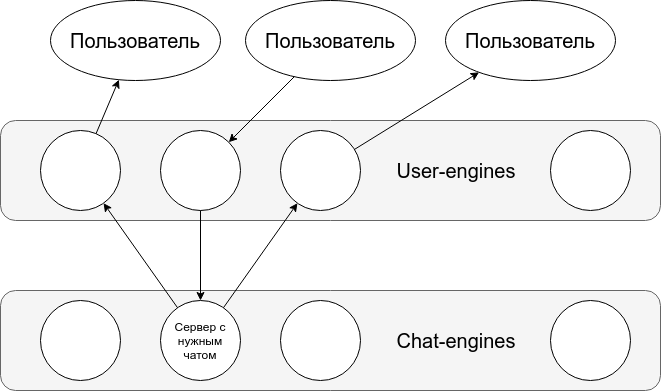
\includegraphics[width=6in]{pics/messages-structure.png}
  \caption{Отправка сообщения во <<В Контакте>>}
  \label{fig10}
\end{figure}


Когда пользователь посылает сообщение, он отправляет его в соответствующий ему user-engine, 
который, зная в какой чат послано сообщение, отправляет его в нужный chat-engine, который в свою
 очередь, рассылает данное сообщение всем участникам чата в нужные user-engine. 
Когда пользователь хочет получить сообщения, он посылает запрос соответствующему ему user-engine, 
который хранит список всех его сообщений с ссылками на нужные чаты. User-engine запрашивает нужные сообщения
 из chat-engine (либо берет их из своего кеша) и отдает пользователю.


Все эти сервисы располагаются на 500 серверах, каждый из которых имеет по 128 гигабайт оперативной
 памяти. На каждом сервере запущено восемь user-engine и восемь chat-engine (по количеству жестких 
 дисков). Каждому user-engine выделено 8 гигабайт оперативной памяти, а каждому chat-engine 4,5 
 гигабайта. Нас интересует способ хранения сообщений в chat-engine. На каждый chat-engine приходится 
 в среднем 500 миллионов сообщений суммарным размером 13 гигабайт. Из 4,5 гигабайт памяти,
 которая выделена chat-engine, он тратит примерно половину на поисковый индекс и хранение метаинформации сообщений.
 На хранение текстов сообщений остается в среднем 2,5 гигабайта.


 Таким образом, если бы удалось сжать сообщения в пять раз, то все сообщения поместились бы в память и 
 не было бы никаких проблем. Но нам не удалось достичь такой степени сжатия, поэтому сообщения подгружаются с диска
 по мере необходимости. Если же свободная память заканчивается, то сообщения чата, которые дольше всего не спрашивали,
 выгружаются из памяти.

 Из описанной архитектуры следует, что самую важную роль при выборе алгоритма сжатия играет общий размер сообщений, 
 который может быть сохранен в памяти.
 При этом следует учитывать, что данная архитектура позволяет сохранить некоторую дополнительную информацию и использовать ее
 при сжатии и разжатии данных. Можно считать, что у алгоритма есть в распоряжении примерно 2,5 гигабайта памяти, которую он 
 может использовать под дополнительную информацию (обозначим ее через $additional\ info$) и хранение сжатых сообщений ($compressed\ size$).
Обозначим суммарный размер исходных сообщений как $messages\ size$, тогда $compress\ ratio = \frac{messages\ size}{compressed\ size + additional\ info}$.
Как раз $compress\ ratio$ нам и нужно оптимизировать. Чем он больше~---тем лучше.

Также важную роль играет скорость, с которой алгоритм может сжимать и разжимает данные. 
Нельзя допустить, чтобы часто случалась ситуация, когда сообщения отдаются пользователю слишком долго. 
Это условие довольно сложно описать формально. Во-первых, чем быстрее средняя скорость сжатия/разжатия, тем лучше.
Но при этом будет плохо, если будет много случаев, когда сообщения отдаются дольше секунды. Также важно не
только время конвертации одного сообщения, но и суммарная нагрузка на процессор, которая создается за счет 
конвертации данных.

\section{Существующие алгоритмы сжатия}

На данный момент существует огромное множество алгоритмов сжатия данных. Нас интересуют только алгоритмы, которые сжимают
данные без потерь. Среди них нас интересуют те, которые ориентированы на сжатие текстовых данных. Далее будут рассмотрены некоторые из них.
Более детально можно ознакомиться с ними в \cite{handbook}.

\subsection{Run-Length encoding}
Кодирование длин серий (или RLE)~--- один из самых простых алгоритмов сжатия данных. Он работает хорошо, если в тексте много подряд идущих одинаковых символов.
Идея алгоритма заключается в том, чтобы заменить $n$ подряд идущих символов $c$ на строку $nc$. Например, строка \text{ABAAACCCCCA} будет заменена на 
\text{1A1B3A5C1A}. 

В показанном примере размер строки уменьшился с 11 символов до 10, однако очень просто привести пример на котором размер строки увеличится. 
Например, строка \text{ABC} превратится в \text{1A1B1C} и станет в два раза длиннее.

Данный метод редко используют на практике для сжатия текстовых данных, однако во многих современных алгоритмах 
сжатия текста используется LZ77, который является обобщением RLE \cite{rle-wiki}.

\subsection{LZ77}

Идея алгоритма заключается в том, чтобы ссылаться на предыдущее вхождение текста. Более формально~--- кодировщик хранит последние несколько килобайт закодированных данных,
а когда хочет закодировать очередной кусок текста, находит наибольшее вхождение текста, которое он помнит, и выписывает пару чисел, которые обозначают как давно он видел
этот текст и какой он длины.

Согласно \cite{lz77-wiki} одним из недостатков данного метода является малая эффективность при кодировании небольшого объема данных. В решаемой нами задаче средняя длина 
сообщения очень маленькая, поэтому алгоритм скорее всего не даст хороших результатов.

\subsection{PPM}

Предсказание по частичному совпадению (Prediction by Partial Matching)~--- алгоритм, который предсказывает вероятность появления очередного символа основываясь на предыдущем опыте.
Параметром модели PPM является число $n$~--- максимальный размер контекста, который анализируется. Обычно $n$ порядка нескольких символов. Для того, чтобы оценить вероятность появления 
конкретной очередной буквы рассматриваются все подстроки длины $n$, которые совпадают с последними $n$ символами. Рассматриваются все символы, которые следуют после найденных подстрок.
Если нужного символа нет, то записывается символ-исключение и рассматривается контекст размера $n - 1$ аналогичным образом. Так происходит пока не найдется подстрока, после которой идет 
нужная буква. Если такой строки найти не удалось, используется контекст степени -1, в котором есть все нужные символы.

К этому алгоритму также применяется следующая оптимизация. Если контекст длины $n$ не подошел, то точно известно, что необходимый символ точно не тот, который мог бы следовать после подстроки 
длины $n$. Поэтому вероятности этих символов при рассмотрении контекста размера $n - 1$ можно прировнять нулю.

Заметим, что данный алгоритм только предсказывает вероятность увидеть очередной символ, но не говорит как нужно кодировать данные.
Поэтому его нужно использовать вместе с алгоритмом энтропийного кодирования. Например, можно использовать алгоритм Хаффмана или арифметическое кодирование.

\subsection{Алгоритм Хаффмана}

Алгоритм Хаффмана~--- алгоритм, который был изобретен в середине прошлого века~\cite{huffman}. Идея заключается в следующем.
Пусть для каждого символа $i$ известна вероятность того, что он сейчас встретится $p_i$. Задача состоит в том,
чтобы сопоставить каждому символу битовую строку $s_i$ и минимизировать $\sum{p_i \cdot |s_i|}$. При этом необходимо,
чтобы не было двух строк таких, что одна является префиксом другой.

Оказывается, что решить эту задачу можно с помощью следующего жадного алгоритма. Рассмотрим два символа с
наименьшими вероятностями. Заменим их на один виртуальный символ, вероятность которого равна сумме вероятностей
исходных символов. Будем повторять этот процесс пока не останется один символ. После этого построим двоичное дерево 
следующим образом. Возьмем единственный символ, он будет корнем дерева. Будем повторять следующую операцию пока возможно.
Рассмотрим лист дерева, который соответствует виртуальному символу. Добавим этой вершине двух детей и скажем, что они
соответствуют символам, из которых была получена текущая виртуальная вершина.

После того как дерево построено, каждому листу в нем соответствует некоторый символ исходного алфавита. Также ему можно сопоставить 
путь из корня до него. Запишем его как битовую строку, в которой переход к левому ребенку соответствует нулю, а к правому~--- единице.
Скажем, что исходному символу соответствует полученная битовая строка.

\subsection{Арифметическое кодирование}

Недостатком алгоритма Хаффмана является то, что он не может закодировать символ нецелым числом бит. Этого недостатка лишено арифметическое кодирование.
Оно работает следующим образом. Каждому сообщению сопоставляется некоторое вещественное число, которое определяется следующим образом. Изначально берется отрезок [0, 1] и разбивается
на столько подотрезков, сколько символов алфавита. При этом размеры отрезков должны быть пропорциональны вероятности получения символа.

Перейдем к отрезку, который соответствует первому символу сообщения, и разобьем его опять в таком же соотношении (либо в другом, если вероятности встретить конкретные символы поменялись).
Перейдем в отрезок, который соответствует второму символу и так далее. После рассмотрения последнего символа выберем вещественное число из отрезка, которое записывается с помощью
наименьшего числа бит. Это и будет закодированное сообщение.

Эффективность такого сжатия строго не хуже алгоритма Хаффмана, а в большинстве случаев превосходит его. Однако, эффективная реализация данного алгоритма достаточно затруднительна. 

\subsection{Современные архиваторы}

Сейчас существует очень много различных архиваторов, но все они основаны на одних и тех же принципах, которые применяются в алгоритмах, описанных выше.
Сейчас стандартом сжатия является Deflate \cite{facebook}, который
используется в zip, gzip, zlib и других архиваторах. Сам алгоритм является смесью LZ77 и алгоритма Хаффмана.

Также интересен алгоритм zstd \cite{zstd-wiki}, который был разработан в Facebook, и сочетает в себе LZ77 и энтропийное кодирование типа Finite State Entropy.

\chapterconclusion

Существует достаточно много алгоритмов сжатия данных без потерь, некоторые из которых были рассмотрены. Поставленная задача существенно отличается от обычной задачи сжатия данных
необходимостью возможности разжимать отельные сообщения. Из-за этого большинство алгоритмов сжатия становятся неприменимы. Некоторые из них можно модифицировать таким образом,
чтобы они решали поставленную задачу. 
\chapter{Разработка алгоритма}

Большинство алгоритмов сжатия обучают свою модель в процессе сжатия текста основываясь на только что полученных данных. 
Исходные данные, которые рассматриваются в нашей задаче, не позволяют так делать, так как данных
 одного сообщения зачастую слишком мало, чтобы заметить в них закономерности. Поэтому необходим алгоритм, 
 который может обучиться на полном наборе сообщений, а потом использовать полученные знания для кодирования 
 отдельных сообщений. При этом полученные знания должны быть сохранены достаточно компактно. 

\section{Однобуквенный Хаффман}
В качестве основы для нашего решения был взят алгоритм Хаффмана~\cite{huffman}, 
так как он позволяет заранее построить модель на исходных данных, а потом использовать ее для сжатия 
отдельных сообщений. Идея  алгоритма достаточно проста. Пусть у нас есть алфавит из $n$ символов. 
Посчитаем $cnt_i$~--- количество раз, которое символ $i$ встречается в исходном наборе сообщений.
 Положим $p_i = \frac{cnt_i}{\sum{cnt_i}}$~--- вероятность встретить символ $i$. Далее каждому символу $i$ ставится 
 в соответствие некоторая битовая строка $s_i$, такая что $\sum\limits_{i} |s_i| \cdot p_i$ как можно меньше и 
  $\forall i \neq j : s_i \text{ не является префиксом } s_j$. Второе условие позволяет однозначно декодировать закодированное
   сообщение, а первое говорит о том, что код является оптимальным среди всех префиксных кодов.
После того как получены строки $s_i$ можно приступать к кодированию. Для этого алгоритм рассматривает все
 символы строки слева направо и заменяет символ $i$ на битовую строку $s_i$.

Чтобы декодировать сообщение алгоритм рассматривает битовую запись полученных данных. Каждый раз
 выбирается строка $s_i$, которая является префиксом еще не декодированных данных, на выход записывается 
 символ $i$, а из исходных данных выкидываются первые $|s_i|$ символов. Заметим, что существует только 
 одна строка $s_i$, которая может быть взята, так как код является префиксным. Чтобы быстро осуществлять
  поиск подходящей строки $s_i$ все строки удобно добавить в структуру данных префиксное дерево \cite{knuth}.

Достоинством этого алгоритма является количество данных, которые ему нужно хранить после обучения 
на исходном наборе сообщений. А именно, единственное, что нужно знать алгоритму, это количество 
вхождений каждой буквы в сообщениях. Если считать, что размер алфавита $256$, а количество вхождений
 хранится в $32$-битном типе данных, то на хранение дополнительной информации потребуется всего $256\times 4 = 1024$ байт = $1$ кбайт.
К сожалению, эффективность сжатия у такого алгоритма не очень высокая. В частности на тестовой 
выборке сообщений был получен коэффициент сжатия 1,37.
 
\section{Хаффман по словам} 
Логичным улучшением этого подхода является изменение алфавита. А именно, в качестве алфавита
 можно использовать не $256$ символов, а, например, слова \cite{handbook}. 
 Предлагается поддерживать два отдельных словаря. Один для того, что называется словами в обычном
  понимании, а другой для знаков препинания и всего остального. При этом в сообщениях слова из
   двух словарей должны строго чередоваться. Также при кодировании необходимо указать из какого 
   словаря взято первое слово. Либо всегда считать, что оно из конкретного словаря, но тогда в 
   него необходимо добавить <<пустое>> слово и, соответственно, подсчитать его вероятность. 
Для разделения на слова и знаки пунктуации будем использовать следующий метод. Разделим все символы, 
которые могут встречаться, на два множества. В первое отнесем большие и маленькие буквы
 (как латинские, так и кириллические), а во второе все остальные. Словом будем считать наибольший 
 по включению набор соседних символов, которые лежат в одном множестве. 

В \cite{handbook} отмечены следующие недостатки данного метода:
\begin{enumerate}
	\item словари достаточно большие. Поэтому они могут не помещаться в память, и для работы с ними нужно 
использовать эффективные алгоритмы;
	\item на входных данных маленького размера практически все слова различны и поэтому алгоритм не успеет 
обучиться;
	\item необходимо два прохода по данным: один чтобы разбить на слова и подсчитать вероятности, второй 
чтобы закодировать;
	\item словарь, посчитанный после первого прохода, необходимо передать декодеру, а он может быть очень 
большим, что сильно ухудшает эффективность сжатия;
	\item слова могут быть сколь угодно длинными, что создает дополнительные проблемы.
\end{enumerate}

Также отмечается, что подобная версия алгоритма Хаффмана дает лучше сжатие чем та, которая сжимает
 отдельные символы, но работает медленнее.

Заметим, что большинство отмеченных недостатков не применимы к нашей задаче. Во-первых, нам в любом 
случае необходимо сделать двухпроходный алгоритм, так как алгоритм должен обучиться на большой выборке
 сообщений. Во-вторых, хоть каждое отдельное сообщение имеет короткую длину, суммарное количество 
 данных очень большое, и поэтому алгоритм сможет посчитать необходимую статистику по встречаемости 
 слов достаточно точно. Что касается больших словарей, то проблема действительно применима к нашей
  задаче и далее будут предложены пути ее решения.

\section{Выбор размера словаря}

Если действовать строго по алгоритму, который описан в \cite{handbook}, то размер словарей действительно получается очень большой. 
Поэтому актуальным является вопрос уменьшения его размера. Легко заметить, что можно выбросить из словаря слова,
которые встречаются в тексте всего один раз, т. к. при записи их в несжатом виде суммарный размер данных не увеличится.
Причем поскольку словарь всегда находится в памяти, а сами сообщения нет, то такое действие окажет точно положительный эффект.

Логичным продолжением данной идеи является выкидывание из словаря слов, которые встречаются меньше чем $K$ раз. Но стает вопрос о том, 
как узнать какое $K$ является оптимальным. Для того, чтобы ответить на этот вопрос нами был создан специальный набор сообщений,
на котором проводилось тестирование. Этот набор состоял из реальных сообщений, которые были посланы пользователями. Каждое сообщение 
попало в этот набор с вероятностью $\frac{1}{200000}=0,000005$, т.е. набор по размеру составляет $2\%$ от сообщений, которые обрабатываются 
одним chat-engine. Суммарный его размер равен 310 мегабайт и в нем содержится 10 миллионов сообщений. В набор были добавлены только непустые
сообщения.

Чтобы узнать правильное значение $K$ был проведен ряд экспериментов. Размер выбранного набора был достаточно маленьким, так как 
время работы алгоритма достаточно большое, а хотелось провести много экспериментов. Но оказалось, что этого достаточно. 
Было проведено 5 групп экспериментов. В них было оставлено $5 \cdot 10^5, 10^6, 2,5 \cdot 10^6, 5 \cdot 10^6, 10^7$ сообщений. В каждой группе был запущен алгоритм
для $K = 1..15$.

В каждом запуске алгоритма нас интересовала степень сжатия данных, а также степень сжатия с учетом словаря. Именно последнюю величину нужно было максимизировать.
На рис.~\ref{fig2},~\ref{fig3},~\ref{fig4} показаны результаты некоторых экспериментов. Как можно заметить, результаты экспериментов для разного количества сообщений очень похожи.
Оказалось, что для всех проведенных экспериментов наилучшим значением $K$ было 8. Т. е. оказалось, что оптимально оставлять в словаре слова, которые встретились в сообщениях
восемь и больше раз вне зависимости от исходного количества сообщений. Разумеется, данная константа справедлива только при достаточно большом количестве сообщений и
только на данных такого же типа как и данные, которые были рассмотрены.

\begin{figure}[h!]
  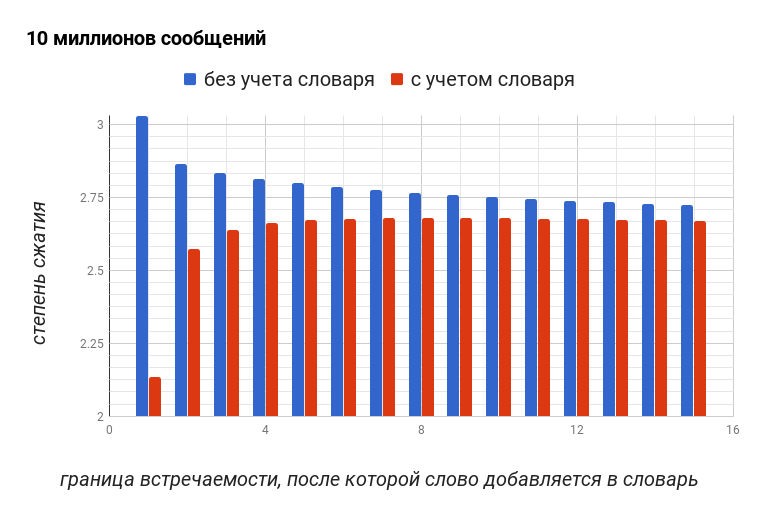
\includegraphics[width=5in]{pics/compress10m.png}
  \caption{Степень сжатия в зависимости от размера словаря (10 миллионов сообщений)}
  \label{fig2}
\end{figure}

\begin{figure}[h!]
  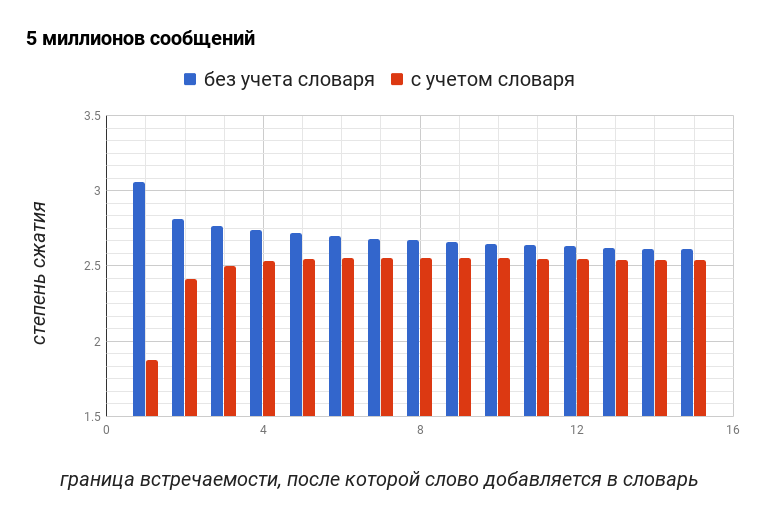
\includegraphics[width=5in]{pics/compress5m.png}
  \caption{Степень сжатия в зависимости от размера словаря (5 миллионов сообщений)}
  \label{fig3}
\end{figure}

\begin{figure}[h!]
  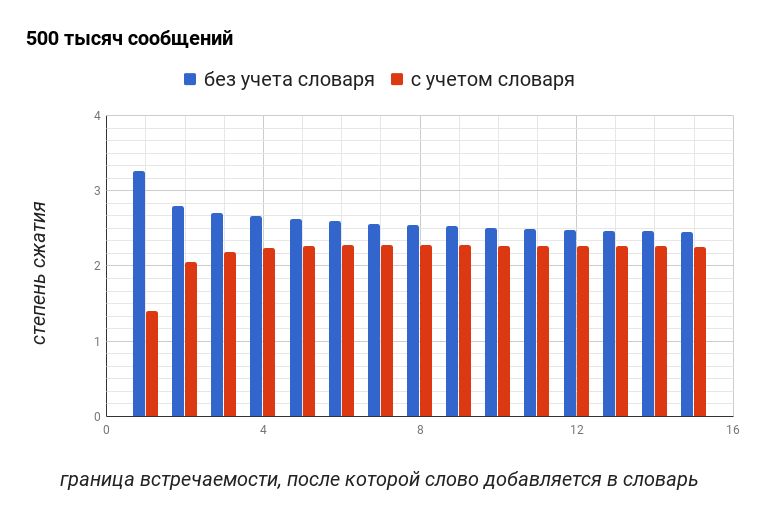
\includegraphics[width=5in]{pics/compress500k.png}
  \caption{Степень сжатия в зависимости от размера словаря (500 тысяч сообщений)}
  \label{fig4}
\end{figure}

Также интересной статистикой является размер словаря, который получается при выборе различных $K$. 
График зависимости количества слов в словаре от того, начиная с какой частоты их добавлять в словарь,
 изображен на рис.~\ref{fig5}. Аналогичный график с размером словаря изображен на рис.~\ref{fig6}. 

\begin{figure}[h!]
  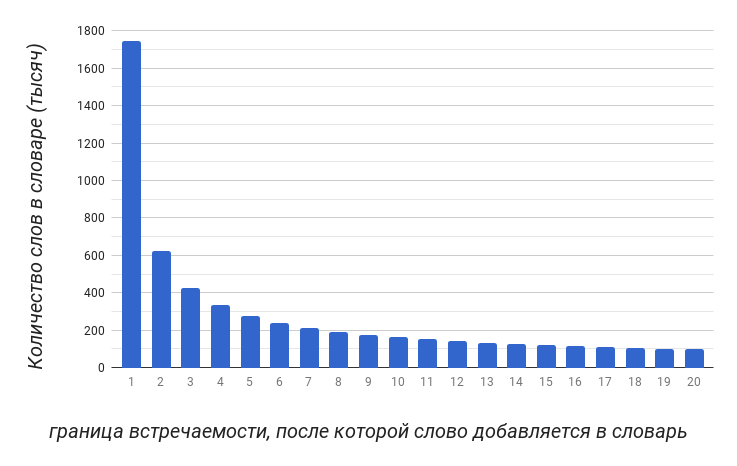
\includegraphics[width=5in]{pics/words_in_dict.png}
  \caption{Количество слов в словаре в зависимости от K}
  \label{fig5}
\end{figure}

\begin{figure}[h!]
  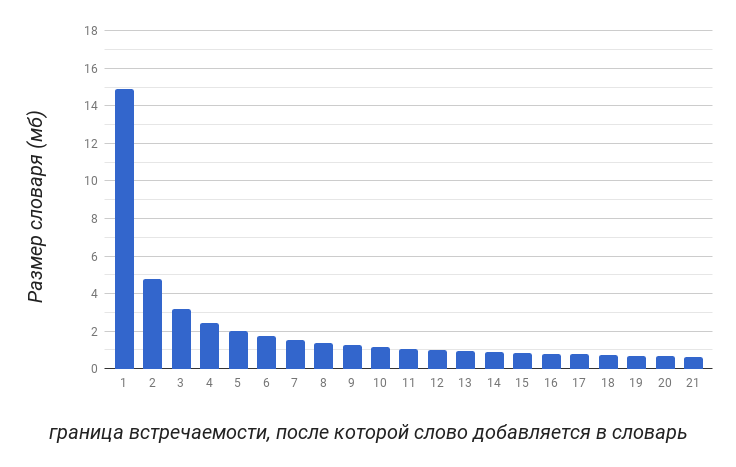
\includegraphics[width=5in]{pics/dict_size.png}
  \caption{Размер словаря в зависимости от K}
  \label{fig6}
\end{figure}

\section{Кодирование слов, которые не попали в словарь}

Описание алгоритма Хаффмана, который оперирует словами, встречается в небольшом количестве источников и во 
всех из них предлагается записывать слова, которые не встретились в словаре, как несжатую последовательность 
байт, предварительно написав символ-исключение. Такой подход разумен в случае, если в словарь добавляются все 
слова, которые встретились в тексте. Однако в нашем подходе для уменьшения размера словаря большое количество
слов исключается из него. Поэтому предлагается сжимать слова не из словаря с помощью какого-нибудь 
другого алгоритма сжатия.

Однако выбор алгоритма для сжатия таких слов не очень прост. Во-первых, алгоритм не должен использовать дополнительную память
или использовать ее мало. Во-вторых, данные для сжатия довольно плохо могут быть сжаты по своей сути. 
Например, мы знаем, что там нет слов, которые встречаются много раз. В-третьих, мы хотим
сжимать отдельные слова, а не связный текст.

Заметим, что обойтись без дополнительной памяти совсем скорее всего не получится, т. к. в отдельном сообщении максимум несколько слов,
которые не попали в словарь, и найти какие-то закономерности алгоритм не успеет.

Достаточно хорошо под критерии подходит обычный алгоритм Хаффмана, который работает с символами. 
Действительно, как было показано ранее, он использует всего один килобайт дополнительной памяти, что очень хорошо нам подходит.
Использование этого алгоритма позволило улучшить коэффициент сжатия с 2,04 до 2,38 на тестовых данных.

\section{Двухсимвольный Хаффман}

Нам хотелось еще больше соптимизировать часть сжатия, которая касается слов, которые не попали в словарь. Для этого был придуман
следующий алгоритм, который основан на обычном алгоритме Хаффмана. 

Большинство алгоритмов сжатия используют контекст, т. е. информацию о том, какие символы были закодированы последними. 
Предлагается сделать тоже самое для алгоритма Хаффмана. А именно, посчитаем $p_{ij}$~---вероятность того, что после буквы $i$ идет буква $j$.
Пусть размер алфавита равен $n$, тогда для каждого символа $i$ построим дерево Хаффмана с $n$ листьями на вероятностях $p_{ij}$. Путь в дереве $i$
до листа $j$ сопоставим строке $s_{ij}$. Алгоритм кодирования данных показан в листинге~\ref{lst1}, а декодирования в листинге~\ref{lst2}.
\begin{algorithm}[!h]
\caption{Кодирование двухсимвольным Хаффманом}\label{lst1}
\begin{algorithmic}
	\Function{Code}{$word$, $s_{ij}$}
		\State $prev \gets 0$
		\State $res \gets \text{empty string}$
		\For{$i\gets 1, len(word)$}
			\State $res \gets res + s_{prev, word[i]}$
			\State $prev \gets word[i]$
		\EndFor
		\State\Return $res$
	\EndFunction
\end{algorithmic}
\end{algorithm}

\begin{algorithm}[!h]
\caption{Декодирование двухсимвольным Хаффманом}\label{lst2}
\begin{algorithmic}
	\Function{Decode}{$encoded$, $s_{ij}, n$}
		\State $it \gets 1$
		\State $res \gets \text{empty string}$
		\State $prev \gets 0$
		\While{$it\le len(encoded)$}
			\For{$i\gets 1, n$}
				\State $len \gets |s_{prev, i}|$
				\If{$encoded[it..it + len - 1] = s_{prev, i}$}
					\State $it\gets it+len$
					\State $res \gets res + i$
					\State $prev \gets i$
					\State \textbf{break}
				\EndIf
			\EndFor
		\EndWhile
		\State\Return $res$
	\EndFunction
\end{algorithmic}
\end{algorithm}

Если при определении, какие слова нужно оставлять в словаре, суммарный размер сообщений почти не играл роли, то на коэффициент сжатия 
он влияет довольно сильно. Это происходит потому что дополнительная информация, необходимая для работы алгоритма, константного размера ($4 \cdot 256 \cdot 256 = 256 \text{ кб}$),
а значит ее относительный размер уменьшается. На рис.~\ref{fig7} показано сравнение коэффициентов сжатия следующих алгоритмов
в зависимости от количества сообщений:
\begin{enumerate}
	\item алгоритм Хаффмана по словам;
	\item алгоритм Хаффмана по словам. Слова, которые не попали в словарь, сжимаются односимвольным Хаффманом;
	\item алгоритм Хаффмана по словам. Слова, которые не попали в словарь, сжимаются двухсимвольным Хаффманом.
\end{enumerate}

\begin{figure}[h!]
  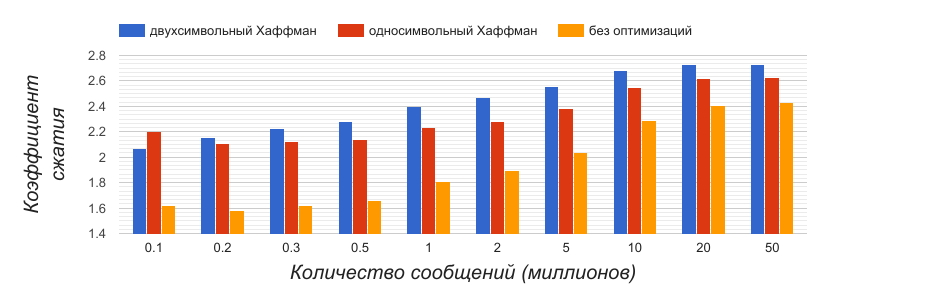
\includegraphics[width=\linewidth]{pics/compare.png}
  \caption{Коэффициент сжатия в зависимости от количества сообщений}
  \label{fig7}
\end{figure}

\section{Реализация алгоритма}

Теперь остановимся более подробно на реализации разработанного алгоритма. Наш алгоритм должен уметь выполнять следующие функции:
\begin{enumerate}
	\item train(String s)~--- использовать сообщение для тренировки;
	\item trainEnd()~--- обучение закончено. Алгоритм должен построить все необходимые ему структуры;
	\item compress(String s)~--- сжать строку. Алгоритм должен вернуть некоторую последовательность байт;
	\item decompress(byte[] data)~--- разжать строку. Алгоритм должен разжать переданные ему данные.
\end{enumerate}

Самое главное свойство алгоритма~--- для любой строки $s$ decompress(compress($s$)) = $s$.

Реализация функций train и compress во многом совпадает. Необходимо разбить исходную строку на составные части, а потом что-то с ними сделать.
Реализация функции split, которая разбивает сообщение на слова, приведена в листинге~\ref{lst3}. Он предполагает, что в коде есть функция $isAlphabetic$, которая отвечает на вопрос о том, 
как делить все символы на два различных множества. В ней нужно учесть кодировку, в которой хранятся данные, а также язык, на котором 
посылаются сообщения. Например во <<В Контакте>> есть много сообщений на украинском языке и необходимо добавить букву `i' в правильное множество.

\begin{algorithm}[!h]
\caption{Алгоритм разбития сообщения на слова}\label{lst3}
\begin{lstlisting}
 public void split(String s) {
 	boolean needAlphabetic = true;
 	for (int i = 0; i < s.length(); ) {
 		int j;
 		while (j != s.length() && isAlphabetic(s.chatAt(j)) == needAlphabetic) {
 			j++;
 		}
 		// do smth with s[i..j]
 		i = j;
 		needAlphabetic = !needAlphabetic;
 	}
}
\end{lstlisting}
\end{algorithm}

Таким образом функция train должна выглядеть также как и split, а внутри добавить слово в словарь, который соответствует $needAlphabetic$.

Функция trainEnd должна выполнить два одинаковых действия с двумя словарями. А именно из него необходимо удалить слова, которые встречаются мало раз.
При этом посчитаем вероятности $p_{ij}$ того, что после символа $i$ следует символ $j$ в этих словах. Кроме того посчитаем суммарную вероятность слов,
которые были удалены, и добавим слово-исключение с такой вероятностью.

Далее построим дерево Хаффмана для оставшихся слов. Кроме того необходимо построить $n$ дополнительных деревьев Хаффмана, где $n$~--- размер алфавита. 
$i$-е такое дерево должно соответствовать символу, который хотим написать после символа $i$. Также необходимо сделать все вероятности ненулевыми, чтобы
иметь возможность записать даже слово, которое раньше не видели.

Также необходимо добавить все слова в хеш-таблицу, в которой по слову можно узнать какое битовое представление ему соответствует.

Теперь рассмотрим реализацию функции compress. Во-первых необходимо аналогично функции split разбить сообщение на слова. Каждое слово необходимо
попытаться найти в хеш-таблице, которая соответствует $needAlphabetic$. Если слово найдено, то запишем его битовую запись и перейдем к следующему слову.
В противном случае необходимо написать слово-исключение, а потом закодировать слово с помощью двухсимвольного Хаффмана, который был описан в листинге~\ref{lst1}.

Функция decompress чуть более сложна в реализации. Она представлена в листинге~\ref{lst4}. Чтобы код не получился слишком громоздким и нечитабельным
были сделаны некоторые допущения:
\begin{enumerate}
	\item существует класс BitStream, который переводит набор байтов в последовательность битов.
	Также он умеет спускаться по переданному ему дереву Хаффмана, читая биты, и вернуть полученный лист дерева;
	\item можно пренебречь тем, что конкатенация строк работает в худшем случае за квадрат от суммарной длины.
	В реальности необходимо использовать StringBuilder;
	\item decodeTwoSybolHuffman~--- функция описанная в листинге~\ref{lst2}. 
	Можно считать, что декодирование происходит до тех пор пока не встречен специальный символ окончания.
\end{enumerate}

\begin{algorithm}[!h]
\caption{Алгоритм декодирования сообщения}\label{lst4}
\begin{lstlisting}
public String decompress(bytes[] data) {
 	String res = "";
 	BitStream bitStream = new BitStream(data);
 	boolean needAlphabetic = true;
 	while (bitStream.hasMoreData()) {
 		Token token = bitStram.readToken(needAlphabetic ? wordsTree : notWordsTree);
 		if (token.isEscapeWord()) {
 			res += decodeTwoSymbolHuffman(bitStream);
 		} else {
 			res += token.getWord();
 		}
 		needAlphabetic = !needAlphabetic;
 	}
 	return res;
}
\end{lstlisting}
\end{algorithm}

\section{Оптимизации}

На практике при реализации описанного алгоритма были применены некоторые оптимизации, 
которые позволили увеличить скорость работы алгоритма.

Рассмотрим функцию BitStream.readToken, которая была использована в листинге~\ref{lst4}. Ее реализация представлена в листинге~\ref{lst5}.
\begin{algorithm}[!h]
\caption{Спуск по дереву Хаффмана}\label{lst5}
\begin{lstlisting}
public Token readToken(TreeNode node) {
 	while (node.left != null) {
 		if (readBit()) {
 			node = node.right;
 		} else {
 			node = node.left;
 		}
 	}
 	return node.getToken();
}
\end{lstlisting}
\end{algorithm}

Такая реализация работает очень долго. У нее есть несколько проблем. 

Во-первых, на каждый бит сжатых данных происходит условный переход. 
Причем процессор не может предсказать в какую именно ветку условия нужно пойти, поскольку переходы по ним происходят примерно одинаково часто 
(за счет того, что это дерево Хаффмана). Это полностью ломает конвейерную обработку запросов процессором, что может ухудшить время работы в
несколько раз.

Во-вторых, на каждый бит сжатых данных происходит переход в случайную ячейку памяти. Поскольку размер деревьев в нашем алгоритме может 
достигать миллиона элементов, такой переход не попадет ни в какой кеш процессора.

Чтобы ускорить время выполнения этой функции была реализована следующая идея. Предподсчитаем, что сделает функция readToken, в зависимости
от того, какие будут результаты выполнения следующих 16 вызовов функции readBit для всех возможных $2^{16}$ вариантов. Существует два варианта:
\begin{enumerate}
	\item функция прочитает не более 16 бит, дойдет до листа в дереве Хаффмана и вернет его;
	\item функция прочитает все 16 бит и остановится в некоторой внутренней вершине дерева.
\end{enumerate}

Также необходимо, чтобы BitStream мог наперед выдать следующие 16 бит сжатых данных. Тогда вместо вызова readToken можно посмотреть в
предподсчитанную таблицу. После этого, если нужно, дочитать оставшиеся биты старым способом. Потом информировать BitStream 
сколько бит действительно было прочитано и вернуть нужный лист дерева.

Такой метод требует дополнительно сотни килобайт памяти, но увеличивает скорость работы в несколько раз.

Аналогично для 256 деревьев двухсимвольного Хаффмана были построены таблицы с предподсчитанными переходами на 8 бит вперед.

Кроме того важно правильно реализовать класс BitStream. В нем необходимо избегать условных переходов везде где только можно.

\chapterconclusion

В данной главе был описан разработанный алгоритм сжатия сообщений, который основан на алгоритме Хаффмана. Был детально рассмотрен вопрос размера словаря,
который необходимо использовать, а также способы кодирования слов, которые не попали в словарь. Были описаны детали реализации алгоритма, 
которые помогают увеличить скорость его работы.
\chapter{Сравнение с существующими решениями}

Разработанный алгоритм сложно сравнивать с другими из-за специфики исходных данных. 
Средняя длина сообщений примерно равна 30 символам, а распределение по длинам показано на рис.~\ref{fig10}.

\begin{figure}[h!]
  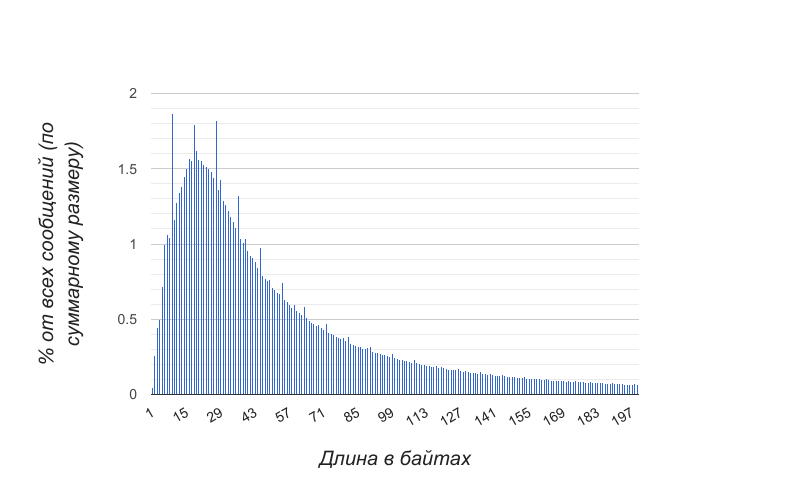
\includegraphics[width=\linewidth]{pics/msgs-len.png}
  \caption{Распределение сообщений по их длинам}
  \label{fig10}
\end{figure}

Проблема заключается в том, что большинство алгоритмов сжатия рассчитаны на сжатие большого объема данных.
В случае же когда сообщения имеют длину порядка 30 байт, то такое сообщение, чаще всего, при сжатии стандартными архиваторами,
станет еще больше. Конечно, можно сжимать сразу весь набор сообщений, но тогда сравнение будет некорректным, так как 
такой метод не позволяет получить произвольное сообщение быстро, а значит решение противоречит поставленной задаче.

Поэтому для сравнения можно брать известные алгоритмы и пытаться модифицировать их так, чтобы они стали применимы к исходной задаче, либо
использовать алгоритмы, которые дают возможность обучиться на некотором наборе данных, а потом использовать полученный словарь, чтобы 
сжимать новые данные.

\section{LZW}
Алгоритм Лемпеля-Зива-Велча (LZW) был опубликован в 1984 году \cite{lzw}.
Идея алгоритма заключается в следующем. Создадим таблицу из слов размера $2^k$ для некоторого $k$. Изначально в нее поместим только отдельные буквы.
Данная таблица будет пополняться по мере кодирования сообщений. Так при кодировании находится наибольшее слово, которое уже есть в словаре, 
записывается позиция этого слова в таблице, а также в таблицу добавляется слово на один большей длины. Значение $k$ при этом может динамически увеличиваться.

Этот алгоритм необходимо было несколько адаптировать под рассматриваемую задачу. А именно, поскольку сообщения короткие, предлагается вначале 
<<прогнать>> алгоритм через все сообщения, чтобы набрать базу слов, а потом кодировать отдельные сообщения с использованием полученной таблицы.
При этом необходимо побороться с тем, что таблица может переполниться. Чтобы такого не произошло будем удалять самые старые слова для освобождения места.

При этом необходимо следить, чтобы не было ситуации, когда некоторое слово есть в таблице, а его префикса нет. Такая ситуация приводит к бесполезной трате оперативной памяти.
Чтобы такого не случалось, необходимо при использовании некоторого слова, переместить все его префиксы в начале LRU (двусвязного списка для удаления старых слов).

Кроме того непонятно, какое значение $k$ использовать. Очевидно, что для маленького количества сообщений необходимо использовать $k$ поменьше, а для большого~--- больше. 
Чтобы определить оптимальное значение было проведено несколько экспериментов с разными $k$.

На рис.~\ref{fig11} показано сравнение разработанного алгоритма и алгоритмов LZW с различными значениями $k$. В качестве набора сообщений для тестов был взят тот же набор,
что описывался в главе про разработку алгоритма.

\begin{figure}[h!]
  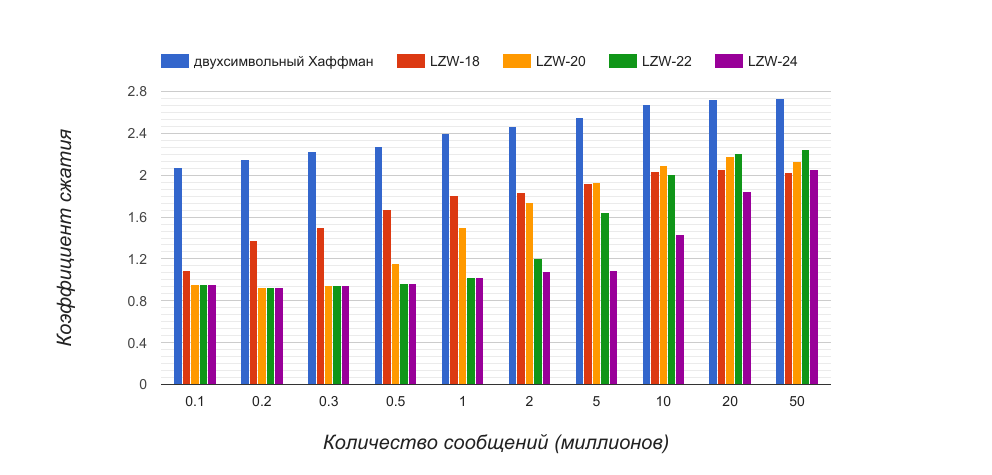
\includegraphics[width=\linewidth]{pics/lzw.png}
  \caption{Сравнение разработанного алгоритма с LZW}
  \label{fig11}
\end{figure}

Как видно из рисунка, разработанный алгоритм достаточно сильно выигрывает у LZW вне зависимости от $k$. Что же касается выбора размера таблицы, то видно,
что на наборах с 20 и 50 миллионами сообщений выигрывает таблица размером $2^{22}$, на 5 и 10 миллионах лучший размер~--- $2^{20}$, а на всех остальных тестах лучше всего
показал себя алгоритм с маленькой таблицей.

\section{SMAZ}

SMAZ~--- одна из немногих библиотек, которые рассчитаны на сжатие коротких текстов \cite{smaz}. В частности, в описании проекта
упоминается, что большинство алгоритмов не могут сжать сообщения длиной меньше 100 символов, а SMAZ может сжать слово \text{the} до одного байта.

Внутри у данного алгоритма фиксированный набор самых часто употребляемых английских слов. Поэтому, если сжимается английский текст, то он может достигнуть 
коэффициента сжатия порядка двух (это все еще значительно меньше чем разработанный нами алгоритм), а на русскоязычных текстах SMAZ не может ничего сжать.

Поскольку smaz рассчитан только на сжатие английских текстов, для сравнения была создана отдельная выборка сообщений. В нее были включены
только сообщения без кириллических символов. Всего было использовано пять миллионов сообщений. Однако, оказалось, что smaz не может сжать эти данные хорошо.
А именно, суммарный размер сообщений после сжатия оказался примерно равным исходному размеру сообщений. 

Такой плохой результат объясняется спецификой сжимаемых данных. Большинство сообщений из набора~--- ссылки и смайлики. А smaz внутри себя содержит 
набор наиболее встречающихся английских слов, которые в данном наборе встречались довольно редко. 

Результаты некоторых других алгоритмов, которые были рассмотрены в работе, показаны в таблице~\ref{tab1}.

\begin{table}[!h]
\caption{Коэффициенты сжатия для сообщений без кириллических символов}\label{tab1}
\centering
\begin{tabular}{|*{2}{c|}}\hline
Алгоритм & Коэффициент сжатия \\\hline
SMAZ & 1,020 \\\hline
Односимвольный Хаффман & 1,389 \\\hline
Хаффман по словам & 1,854 \\\hline
LZW & 2,022 \\\hline
Хаффман по словам + односимвольный Хаффман & 2,282 \\\hline
Хаффман по словам + двухсимвольный Хаффман & 2,391 \\\hline
\end{tabular}
\end{table}

Поскольку на сообщениях пользователей <<В Контакте>> алгоритм smaz показал себя очень плохо, было проведено сравнения алгоритма на обычном английском тексте.
Для этого были использованы тексты книг на английском языке из проекта <<Гутенберг>>~\cite{gutenberg}. Сам текст был разбит на сообщения длиной порядка 40 символов.
Суммарный размер сообщений 6,5 мегабайт, а всего их было 150 тысяч. На таких данных smaz смог достигнуть коэффициента сжатия 1,728, что уже достаточно хорошо,
но все равно уступает разработанному алгоритму. Сравнение алгоритмов представлено в таблице~\ref{tab2}. Заметим, что двухсимвольный Хаффман
показал себя хуже чем односимвольный, так как суммарный размер сообщений слишком маленький.

\begin{table}[!h]
\caption{Коэффициенты сжатия для проекта Гутенберг}\label{tab2}
\centering
\begin{tabular}{|*{2}{c|}}\hline
Алгоритм & Коэффициент сжатия \\\hline
Односимвольный Хаффман & 1,726 \\\hline
SMAZ & 1,728 \\\hline
LZW & 1,957 \\\hline
Хаффман по словам & 2,614 \\\hline
Хаффман по словам + двухсимвольный Хаффман & 2,676 \\\hline
Хаффман по словам + односимвольный Хаффман & 2,936 \\\hline
\end{tabular}
\end{table}


\section{zstd}

Довольно интересным является алгоритм zstd, предложенный Facebook \cite{facebook}. Кроме того,
что он имеет хороший коэффициент сжатия и скорость, он также имеет возможность обучаться на выборке сообщений.

В описании алгоритма есть целый раздел про дополнительное обучение алгоритма, в котором сказано, что оно помогает существенно улучшить степень сжатия JSON размером порядка килобайта.

Сравнение алгоритмов проводилось на выборке из пяти миллионов сообщений, суммарный размер которых 128 мегабайт. Для тренировки алгоритма zstd все сообщений необходимо сохранить в виде отдельных файлов, а потом передать их в качестве аргументов запуска. Из-за ограничения на количество передаваемых аргументов и скорости работы операционной системы с большим количеством маленьких файлов, было 
решено соединить сообщения в группы и сжимать целыми группами.

В качестве первого эксперимента сообщения были собраны по сто штук в группу. После обучения на них zstd сгенерировал словарь размером 112 килобайт. После этого с помощью алгоритма были сжаты исходные сообщения. Суммарный их размер равен 64 мегабайта, а коэффициент сжатия 2,034. Если же сжимать сообщения с помощью zstd, но без словаря, получается коэффициент сжатия 1,675.

Для следующего эксперимента было взято 500 тысяч сообщений суммарным размером 18 мегабайт. При попытке сжать их без словаря был получен коэффициент сжатия 1,169. При сжатии же со словарем коэффициент 
сжатия оказался 1,543.

Кроме того, если сжать все сообщений сразу, не разбивая их на группы, то коэффициент сжатия получается 2,865 (при максимальном уровне сжатия). Этот результат превосходит результат полученный 
с помощью разработанного алгоритма на этих данных (2,531), но, учитывая исходную постановку задачи, не применим, так как в таком виде нельзя разжимать отдельные сообщения. 

Также были проведены некоторые другие эксперименты из которых можно сделать следующие выводы:
\begin{enumerate}
	\item использование словаря улучшает качество сжатия довольно сильно;
	\item чем больше средний размер сообщения, тем лучше коэффициент сжатия;
	\item при среднем размере сообщения порядка нескольких килобайт, коэффициент сжатия становится больше двух и алгоритм приближается по эффективности к разработанному;
	\item при среднем размере сообщений порядка десятка байт, что характерно изучаемым данным, алгоритм zstd применять смысла нет.	
\end{enumerate}

\section{Сравнение на сообщениях из twitter}

Чтобы проверить, что разработанный алгоритм можно применять не только для сжатия конкретного типа сообщений, характерных для ООО <<В Контакте>>, были проведены дополнительные тесты.
В частности, алгоритм был протестирован на случайных русскоязычных сообщениях, полученных с помощью twitter streaming api.

Всего в выборке было три миллиона сообщений, суммарным размером 256 мегабайт. Таким образом средняя длина сообщения превышает среднюю длину для сообщений из <<В Контакте>> и равна 90 символов.

Коэффициенты сжатия, полученные на этих данных, представлены в таблице~\ref{tab3}.

\begin{table}[!h]
\caption{Коэффициенты сжатия для сообщений из twitter}\label{tab3}
\centering
\begin{tabular}{|*{2}{c|}}\hline
Алгоритм & Коэффициент сжатия \\\hline
Односимвольный Хаффман & 1.374 \\\hline
LZW & 2.138 \\\hline
Хаффман по словам & 2.573 \\\hline
Хаффман по словам + односимвольный Хаффман & 2.725 \\\hline
Хаффман по словам + двухсимвольный Хаффман & 2.815 \\\hline
\end{tabular}
\end{table}

\chapterconclusion

В данной главе было проведено сравнение разработанного алгоритма с некоторыми другими алгоритмами. В частности было проведено сравнение с алгоритмом LZW, который был
модифицирован специально для сжатия коротких сообщений. Кроме того было проведено сравнение с существующим архиватором SMAZ, который разрабатывался специально
для сжатия коротких сообщений. Также было проведено сравнение с архиватором zstd, который был разработан в Facebook, и который умеет обучаться на выборке сообщений.
Все алгоритмы, которые были рассмотрены, проигрывают по эффективности разработанному алгоритму.
\startconclusionpage

Был разработан алгоритм сжатия коротких текстовых сообщений. Он основан на алгоритме Хаффмана. Был детально рассмотрен вопрос о размере получаемого словаря и то, как кодировать слова, которые в него не попали. Разработанный метод был детально описан.

Разработанный алгоритм был применен для сжатия сообщений в ООО <<В Контакте>>, что позволило сократить их размер на 5-7\% по сравнению с предыдущей версией сжатия. Такое улучшение в масштабах <<В Контакте>> соответсвует экономии нескольких терабайт оперативной памяти.

Разработанный алгоритм сложно сравнивать с существующими алгоритмами сжатия, так как они не расчитаны на сжатие коротких сообщений. Все найденные решения проигрывают разработанному алгоритму по степени сжатия.

Разработанный алгоритм, а также все дополнительные материалы, доступны в \cite{github}.

Как одно из направлений развития алгоритма можно попробовать использовать арифметическое кодирование вместо алгоритма Хаффмана.

\printmainbibliography

\end{document}
